\documentclass[dvips,10pt]{article}
\usepackage{graphicx}
\setlength{\oddsidemargin}{-0.3in}
\setlength{\textwidth}{7.0in}
\setlength{\topmargin}{-0.70in}
\setlength{\textheight}{9.5in}
\pagestyle{myheadings}
\markright{ {\rm {
GLND DSMB Report-Recruitment, Baseline, and Follow-up OPEN SESSION
 \hspace{2em}
Thu Sep 09 10:22:31 EDT 2010
\hfill
\hspace{3em}
}}}
\headsep=0.2in
\begin{document}
\vspace*{1in}
\begin{center}
{\Huge{CONFIDENTIAL}}
\end{center}
\vspace*{0.5in}
\begin{center}
{\Huge{Efficacy and Mechanisms of GLN Dipeptide in the SICU GLND Trial}}
\end{center}
\vspace*{0.5in}
\begin{center}
{\Huge{Data Safety Monitoring Board Report}}
\end{center}
\vspace*{0.25in}
\begin{center}
{\Huge{
Recruitment, Baseline, and Follow-up  OPEN SESSION
}}
\end{center}
\vspace*{1in}
\begin{center}
{\Huge{GLND DSMB Meeting}}
\end{center}
\begin{center}
{\Huge{
 March 31, 2010
}}
\end{center}
\begin{center}
{\Huge{2-4 pm EDT}}
\end{center}
\vspace*{1in}
\begin{center}
\noindent
{\Large{Includes patients enrolled and follow-up data received as of March 03, 2010}}
\end{center}
\vspace*{0.5in}
\begin{center}
{\Large{Report prepared  Thu Sep 09 10:22:31 EDT 2010 }}
\end{center}
\clearpage
\vspace*{1in}
\begin{center}
{\Huge{Table of Contents}}
\end{center}
\listoftables
\listoffigures
\clearpage
\begin{table}[t]
\caption
{ Patient Screening and Enrollment. }
\begin{center}
\begin{tabular}{ @{}l@{}
@{}l@{}@{}p{1.5em}@{}@{}c@{}@{}p{1.5em}@{}@{}c@{}@{}p{1.5em}@{}@{}c@{}@{}p{1.5em}@{}@{}c@{}
}
\hline

& \parbox{6em}{\begin{center}Clinical Center\end{center}} && \parbox{6em}{\begin{center}No. Screened\end{center}} && \parbox{6em}{\begin{center}No. Eligible (\%)\end{center}} && \parbox{6em}{\begin{center}No. Enrolled (\%)\end{center}} && \parbox{6em}{\begin{center}Date IRB Approved\end{center}} \\

\hline

\\
& Emory && 337 && 62 ( 18\%) && 46 ( 74\%) && 11/01/06 \\
& Miriam && 51 && 22 ( 43\%) && 9 ( 41\%) && 01/01/07 \\
& Vanderbilt && 276 && 48 ( 17\%) && 30 ( 63\%) && 01/01/07 \\
& Colorado && 139 && 27 ( 19\%) && 25 ( 93\%) && 02/01/07 \\
& Wisconsin && 20 && 1 (  5\%) && 1 (100\%) && 11/02/09 \\
& Total && 823 && 160 ( 19\%) && 111 ( 69\%) && . \\
\\
\hline \\

\end{tabular}

\end{center}
 \end{table}
\begin{table}[t]
\caption
{ Recruitment in the last 6 months. }
\begin{center}
\begin{tabular}{ @{}l@{}
@{}c@{}@{}p{1.5em}@{}@{}c@{}@{}p{1.5em}@{}@{}c@{}
}
\hline

& \parbox{6em}{\begin{center}Month\end{center}} && \parbox{6em}{\begin{center}Patients Recruited\end{center}} && \parbox{6em}{\begin{center}Total Recruited\end{center}} \\

\hline

\\
& OCT09 && 2 && 102 \\
& NOV09 && 1 && 103 \\
& DEC09 && 2 && 105 \\
& JAN10 && 3 && 108 \\
& FEB10 && 3 && 111 \\
& MAR10 && 0 && 111 \\
\\
\hline \\

\end{tabular}

\end{center}
 \end{table}

\begin{figure}
\resizebox{6.5in}{!}{\rotatebox{90}{\includegraphics{recruitment.ps}}}
\caption{Recruitment Projections}
\end{figure}

\begin{figure}
\resizebox{7.75in}{!}{\rotatebox{90}{\includegraphics{rc.ps}}}
\caption{Recruitment Projections by Center}
\end{figure}
\clearpage

\begin{figure}
\resizebox{7.75in}{!}{\rotatebox{90}{\includegraphics{rc5.ps}}}
\caption{Recruitment Projections by Center}
\end{figure}
\clearpage
\begin{table}[t]
\caption
{ Patient Screening and Enrollment Within Last 6 months. }
\begin{center}
\begin{tabular}{ @{}l@{}
@{}l@{}@{}p{1.5em}@{}@{}c@{}@{}p{1.5em}@{}@{}c@{}@{}p{1.5em}@{}@{}c@{}@{}p{1.5em}@{}@{}c@{}
}
\hline

& \parbox{6em}{\begin{center}Month\end{center}} && \parbox{6em}{\begin{center}Clinical Center\end{center}} && \parbox{6em}{\begin{center}No. Screened\end{center}} && \parbox{6em}{\begin{center}No. Eligible (\%)\end{center}} && \parbox{6em}{\begin{center}No. Enrolled (\%)\end{center}} \\

\hline

\\
& SEP2009 && Emory && 11 && 1 (  9\%) && 1 (100\%) \\
&  && Miriam && 0 && - && - \\
&  && Vanderbilt && 9 && 4 ( 44\%) && 1 ( 25\%) \\
&  && Colorado && 3 && 0 (  0\%) && - \\
&  && Total && 23 && 5 ( 22\%) && 2 ( 40\%) \\
&  &&  &&  &&  &&  \\
& OCT2009 && Emory && 10 && 1 ( 10\%) && 1 (100\%) \\
&  && Miriam && 0 && - && - \\
&  && Vanderbilt && 8 && 1 ( 13\%) && 1 (100\%) \\
&  && Colorado && 3 && 0 (  0\%) && - \\
&  && Total && 21 && 2 ( 10\%) && 2 (100\%) \\
&  &&  &&  &&  &&  \\
& NOV2009 && Emory && 8 && 0 (  0\%) && - \\
&  && Vanderbilt && 6 && 0 (  0\%) && - \\
&  && Colorado && 1 && 1 (100\%) && 1 (100\%) \\
&  && Wisconsin && 2 && 0 (  0\%) && - \\
&  && Total && 17 && 1 (  6\%) && 1 (100\%) \\
&  &&  &&  &&  &&  \\
& DEC2009 && Emory && 7 && 1 ( 14\%) && 1 (100\%) \\
&  && Vanderbilt && 10 && 1 ( 10\%) && 0 (  0\%) \\
&  && Colorado && 3 && 1 ( 33\%) && 1 (100\%) \\
&  && Wisconsin && 4 && 0 (  0\%) && - \\
&  && Total && 24 && 3 ( 13\%) && 2 ( 67\%) \\
&  &&  &&  &&  &&  \\
& JAN2010 && Emory && 10 && 1 ( 10\%) && 1 (100\%) \\
&  && Vanderbilt && 9 && 2 ( 22\%) && 2 (100\%) \\
&  && Colorado && 1 && 0 (  0\%) && - \\
&  && Wisconsin && 6 && 0 (  0\%) && - \\
&  && Total && 26 && 3 ( 12\%) && 3 (100\%) \\
&  &&  &&  &&  &&  \\
& FEB2010 && Emory && 8 && 0 (  0\%) && - \\
&  && Vanderbilt && 10 && 1 ( 10\%) && 1 (100\%) \\
&  && Colorado && 2 && 1 ( 50\%) && 1 (100\%) \\
&  && Wisconsin && 7 && 1 ( 14\%) && 1 (100\%) \\
&  && Total && 27 && 3 ( 11\%) && 3 (100\%) \\
&  &&  &&  &&  &&  \\
\\
\hline \\

\end{tabular}

\end{center}
 \end{table}
\begin{table}[tbp]
\caption
{ Reasons Patients Were Ineligible at Screening (Emory). }
\begin{center}
\begin{tabular}{ @{}l@{}
@{}c@{}
}
\hline

& \parbox{6em}{\begin{center}Total\end{center}} \\
 & n=355 \\
 \cline{2-2} 
 Characteristic &
 \makebox[1.5em]{n}\makebox[3.5em][r]{(\%)} \\
 \hline
\\
\parbox[b]{ 70mm }{\raggedright{{\bf Reason Not Eligible }}} &
  \\
 \hspace{1em} AGE not 18-80 &
 \makebox[1.5em][r]{5}\makebox[3.5em][r]{(1.4)} \\
 \hspace{1em} BMI $ \ge $ 40 &
 \makebox[1.5em][r]{24}\makebox[3.5em][r]{(6.8)} \\
 \hspace{1em} Burn Trauma Injury &
 \makebox[1.5em][r]{3}\makebox[3.5em][r]{(0.8)} \\
 \hspace{1em} Central Venous PN $<$ 7 days &
 \makebox[1.5em][r]{2}\makebox[3.5em][r]{(0.6)} \\
 \hspace{1em} Cirrhosis or Bilirubin $ \ge $10 &
 \makebox[1.5em][r]{24}\makebox[3.5em][r]{(6.8)} \\
 \hspace{1em} Clinical Sepsis within 24 hrs study entry &
 \makebox[1.5em][r]{7}\makebox[3.5em][r]{(2.0)} \\
 \hspace{1em} Ent/Parent Feedings &
 \makebox[1.5em][r]{16}\makebox[3.5em][r]{(4.5)} \\
 \hspace{1em} Gastric Surgery or Whipple &
 \makebox[1.5em][r]{11}\makebox[3.5em][r]{(3.1)} \\
 \hspace{1em} History of HIV/AIDS &
 \makebox[1.5em][r]{3}\makebox[3.5em][r]{(0.8)} \\
 \hspace{1em} Malignancy &
 \makebox[1.5em][r]{73}\makebox[3.5em][r]{(20.6)} \\
 \hspace{1em} NOT in Post Op Days Range &
 \makebox[1.5em][r]{37}\makebox[3.5em][r]{(10.4)} \\
 \hspace{1em} No Central Access &
 \makebox[1.5em][r]{7}\makebox[3.5em][r]{(2.0)} \\
 \hspace{1em} Organ Transplant &
 \makebox[1.5em][r]{19}\makebox[3.5em][r]{(5.4)} \\
 \hspace{1em} Received Investigational Drug &
 \makebox[1.5em][r]{13}\makebox[3.5em][r]{(3.7)} \\
 \hspace{1em} Received PN 4+ days &
 \makebox[1.5em][r]{2}\makebox[3.5em][r]{(0.6)} \\
 \hspace{1em} Renal Dysfunction &
 \makebox[1.5em][r]{74}\makebox[3.5em][r]{(20.8)} \\
 \hspace{1em} Require PN$<$7 days &
 \makebox[1.5em][r]{15}\makebox[3.5em][r]{(4.2)} \\
 \hspace{1em} Seizure Hist/Disorder &
 \makebox[1.5em][r]{16}\makebox[3.5em][r]{(4.5)} \\
 \hspace{1em} Unexplained Encephalopathy &
 \makebox[1.5em][r]{4}\makebox[3.5em][r]{(1.1)} \\
 \vspace{0em} \\
\hline \\ 
\end{tabular}

\parbox{ 5in }{ *n represents total number of reasons given for ineligible patients } \\
 \vspace{1em}\end{center}
 \end{table}
\begin{table}[tbp]
\caption
{ Reasons Patients Were Ineligible at Screening (Miriam). }
\begin{center}
\begin{tabular}{ @{}l@{}
@{}c@{}
}
\hline

& \parbox{6em}{\begin{center}Total\end{center}} \\
 & n=40 \\
 \cline{2-2} 
 Characteristic &
 \makebox[1.5em]{n}\makebox[3.5em][r]{(\%)} \\
 \hline
\\
\parbox[b]{ 70mm }{\raggedright{{\bf Reason Not Eligible }}} &
  \\
 \hspace{1em} AGE not 18-80 &
 \makebox[1.5em][r]{3}\makebox[3.5em][r]{(7.5)} \\
 \hspace{1em} BMI $ \ge $ 40 &
 \makebox[1.5em][r]{4}\makebox[3.5em][r]{(10.0)} \\
 \hspace{1em} Cirrhosis or Bilirubin $ \ge $10 &
 \makebox[1.5em][r]{3}\makebox[3.5em][r]{(7.5)} \\
 \hspace{1em} Clinical Sepsis within 24 hrs study entry &
 \makebox[1.5em][r]{2}\makebox[3.5em][r]{(5.0)} \\
 \hspace{1em} Gastric Surgery or Whipple &
 \makebox[1.5em][r]{2}\makebox[3.5em][r]{(5.0)} \\
 \hspace{1em} History of HIV/AIDS &
 \makebox[1.5em][r]{1}\makebox[3.5em][r]{(2.5)} \\
 \hspace{1em} Malignancy &
 \makebox[1.5em][r]{10}\makebox[3.5em][r]{(25.0)} \\
 \hspace{1em} No Central Access &
 \makebox[1.5em][r]{1}\makebox[3.5em][r]{(2.5)} \\
 \hspace{1em} Received PN 4+ days &
 \makebox[1.5em][r]{2}\makebox[3.5em][r]{(5.0)} \\
 \hspace{1em} Renal Dysfunction &
 \makebox[1.5em][r]{10}\makebox[3.5em][r]{(25.0)} \\
 \hspace{1em} Require PN$<$7 days &
 \makebox[1.5em][r]{1}\makebox[3.5em][r]{(2.5)} \\
 \hspace{1em} Seizure Hist/Disorder &
 \makebox[1.5em][r]{1}\makebox[3.5em][r]{(2.5)} \\
 \vspace{0em} \\
\hline \\ 
\end{tabular}
\end{center}
 \end{table}
\begin{table}[tbp]
\caption
{ Reasons Patients Were Ineligible at Screening (Vanderbilt). }
\begin{center}
\begin{tabular}{ @{}l@{}
@{}c@{}
}
\hline

& \parbox{6em}{\begin{center}Total\end{center}} \\
 & n=270 \\
 \cline{2-2} 
 Characteristic &
 \makebox[1.5em]{n}\makebox[3.5em][r]{(\%)} \\
 \hline
\\
\parbox[b]{ 70mm }{\raggedright{{\bf Reason Not Eligible }}} &
  \\
 \hspace{1em} AGE not 18-80 &
 \makebox[1.5em][r]{4}\makebox[3.5em][r]{(1.5)} \\
 \hspace{1em} BMI $ \ge $ 40 &
 \makebox[1.5em][r]{35}\makebox[3.5em][r]{(13.0)} \\
 \hspace{1em} Burn Trauma Injury &
 \makebox[1.5em][r]{3}\makebox[3.5em][r]{(1.1)} \\
 \hspace{1em} Central Venous PN $<$ 7 days &
 \makebox[1.5em][r]{8}\makebox[3.5em][r]{(3.0)} \\
 \hspace{1em} Cirrhosis or Bilirubin $ \ge $10 &
 \makebox[1.5em][r]{8}\makebox[3.5em][r]{(3.0)} \\
 \hspace{1em} Clinical Sepsis within 24 hrs study entry &
 \makebox[1.5em][r]{15}\makebox[3.5em][r]{(5.6)} \\
 \hspace{1em} Ent/Parent Feedings &
 \makebox[1.5em][r]{8}\makebox[3.5em][r]{(3.0)} \\
 \hspace{1em} Gastric Surgery or Whipple &
 \makebox[1.5em][r]{5}\makebox[3.5em][r]{(1.9)} \\
 \hspace{1em} In SICU due to wrong reason &
 \makebox[1.5em][r]{18}\makebox[3.5em][r]{(6.7)} \\
 \hspace{1em} Malignancy &
 \makebox[1.5em][r]{67}\makebox[3.5em][r]{(24.8)} \\
 \hspace{1em} NOT in Post Op Days Range &
 \makebox[1.5em][r]{20}\makebox[3.5em][r]{(7.4)} \\
 \hspace{1em} Organ Transplant &
 \makebox[1.5em][r]{10}\makebox[3.5em][r]{(3.7)} \\
 \hspace{1em} Received Investigational Drug &
 \makebox[1.5em][r]{2}\makebox[3.5em][r]{(0.7)} \\
 \hspace{1em} Received PN 4+ days &
 \makebox[1.5em][r]{1}\makebox[3.5em][r]{(0.4)} \\
 \hspace{1em} Renal Dysfunction &
 \makebox[1.5em][r]{32}\makebox[3.5em][r]{(11.9)} \\
 \hspace{1em} Require PN$<$7 days &
 \makebox[1.5em][r]{17}\makebox[3.5em][r]{(6.3)} \\
 \hspace{1em} Seizure Hist/Disorder &
 \makebox[1.5em][r]{16}\makebox[3.5em][r]{(5.9)} \\
 \hspace{1em} Unexplained Encephalopathy &
 \makebox[1.5em][r]{1}\makebox[3.5em][r]{(0.4)} \\
 \vspace{0em} \\
\hline \\ 
\end{tabular}
\end{center}
 \end{table}
\begin{table}[tbp]
\caption
{ Reasons Patients Were Ineligible at Screening (Colorado). }
\begin{center}
\begin{tabular}{ @{}l@{}
@{}c@{}
}
\hline

& \parbox{6em}{\begin{center}Total\end{center}} \\
 & n=148 \\
 \cline{2-2} 
 Characteristic &
 \makebox[1.5em]{n}\makebox[3.5em][r]{(\%)} \\
 \hline
\\
\parbox[b]{ 70mm }{\raggedright{{\bf Reason Not Eligible }}} &
  \\
 \hspace{1em} AGE not 18-80 &
 \makebox[1.5em][r]{1}\makebox[3.5em][r]{(0.7)} \\
 \hspace{1em} BMI $ \ge $ 40 &
 \makebox[1.5em][r]{5}\makebox[3.5em][r]{(3.4)} \\
 \hspace{1em} Burn Trauma Injury &
 \makebox[1.5em][r]{1}\makebox[3.5em][r]{(0.7)} \\
 \hspace{1em} Central Venous PN $<$ 7 days &
 \makebox[1.5em][r]{2}\makebox[3.5em][r]{(1.4)} \\
 \hspace{1em} Cirrhosis or Bilirubin $ \ge $10 &
 \makebox[1.5em][r]{15}\makebox[3.5em][r]{(10.1)} \\
 \hspace{1em} Clinical Sepsis within 24 hrs study entry &
 \makebox[1.5em][r]{2}\makebox[3.5em][r]{(1.4)} \\
 \hspace{1em} Ent/Parent Feedings &
 \makebox[1.5em][r]{2}\makebox[3.5em][r]{(1.4)} \\
 \hspace{1em} Gastric Surgery or Whipple &
 \makebox[1.5em][r]{7}\makebox[3.5em][r]{(4.7)} \\
 \hspace{1em} History of HIV/AIDS &
 \makebox[1.5em][r]{2}\makebox[3.5em][r]{(1.4)} \\
 \hspace{1em} In SICU due to wrong reason &
 \makebox[1.5em][r]{2}\makebox[3.5em][r]{(1.4)} \\
 \hspace{1em} Malignancy &
 \makebox[1.5em][r]{70}\makebox[3.5em][r]{(47.3)} \\
 \hspace{1em} NOT in Post Op Days Range &
 \makebox[1.5em][r]{4}\makebox[3.5em][r]{(2.7)} \\
 \hspace{1em} Organ Transplant &
 \makebox[1.5em][r]{6}\makebox[3.5em][r]{(4.1)} \\
 \hspace{1em} Patient Pregnant &
 \makebox[1.5em][r]{1}\makebox[3.5em][r]{(0.7)} \\
 \hspace{1em} Physician(s) Will NOT Allow &
 \makebox[1.5em][r]{3}\makebox[3.5em][r]{(2.0)} \\
 \hspace{1em} Received Investigational Drug &
 \makebox[1.5em][r]{2}\makebox[3.5em][r]{(1.4)} \\
 \hspace{1em} Received PN 4+ days &
 \makebox[1.5em][r]{1}\makebox[3.5em][r]{(0.7)} \\
 \hspace{1em} Renal Dysfunction &
 \makebox[1.5em][r]{12}\makebox[3.5em][r]{(8.1)} \\
 \hspace{1em} Require PN$<$7 days &
 \makebox[1.5em][r]{2}\makebox[3.5em][r]{(1.4)} \\
 \hspace{1em} Seizure Hist/Disorder &
 \makebox[1.5em][r]{7}\makebox[3.5em][r]{(4.7)} \\
 \hspace{1em} Unexplained Encephalopathy &
 \makebox[1.5em][r]{1}\makebox[3.5em][r]{(0.7)} \\
 \vspace{0em} \\
\hline \\ 
\end{tabular}
\end{center}
 \end{table}
\begin{table}[tbp]
\caption
{ Reasons Patients Were Ineligible at Screening (Wisconsin). }
\begin{center}
\begin{tabular}{ @{}l@{}
@{}c@{}
}
\hline

& \parbox{6em}{\begin{center}Total\end{center}} \\
 & n=27 \\
 \cline{2-2} 
 Characteristic &
 \makebox[1.5em]{n}\makebox[3.5em][r]{(\%)} \\
 \hline
\\
\parbox[b]{ 70mm }{\raggedright{{\bf Reason Not Eligible }}} &
  \\
 \hspace{1em} AGE not 18-80 &
 \makebox[1.5em][r]{1}\makebox[3.5em][r]{(3.7)} \\
 \hspace{1em} BMI $ \ge $ 40 &
 \makebox[1.5em][r]{4}\makebox[3.5em][r]{(14.8)} \\
 \hspace{1em} Burn Trauma Injury &
 \makebox[1.5em][r]{2}\makebox[3.5em][r]{(7.4)} \\
 \hspace{1em} Cirrhosis or Bilirubin $ \ge $10 &
 \makebox[1.5em][r]{2}\makebox[3.5em][r]{(7.4)} \\
 \hspace{1em} Clinical Sepsis within 24 hrs study entry &
 \makebox[1.5em][r]{3}\makebox[3.5em][r]{(11.1)} \\
 \hspace{1em} Ent/Parent Feedings &
 \makebox[1.5em][r]{1}\makebox[3.5em][r]{(3.7)} \\
 \hspace{1em} Malignancy &
 \makebox[1.5em][r]{6}\makebox[3.5em][r]{(22.2)} \\
 \hspace{1em} Physician(s) Will NOT Allow &
 \makebox[1.5em][r]{1}\makebox[3.5em][r]{(3.7)} \\
 \hspace{1em} Renal Dysfunction &
 \makebox[1.5em][r]{4}\makebox[3.5em][r]{(14.8)} \\
 \hspace{1em} Require PN$<$7 days &
 \makebox[1.5em][r]{2}\makebox[3.5em][r]{(7.4)} \\
 \hspace{1em} Seizure Hist/Disorder &
 \makebox[1.5em][r]{1}\makebox[3.5em][r]{(3.7)} \\
 \vspace{0em} \\
\hline \\ 
\end{tabular}
\end{center}
 \end{table}
\clearpage
\begin{table}[t]
\caption
{ Reasons Patients Eligible at Screening Were Not Enrolled. }
\begin{center}
\begin{tabular}{ @{}l@{}
@{}l@{}@{}p{1.5em}@{}@{}c@{}@{}p{1.5em}@{}@{}l@{}
}
\hline

& \parbox{6em}{\begin{center}Clinical Center\end{center}} && \parbox{6em}{\begin{center}GLND ID No.\end{center}} && \parbox{6em}{\begin{center}Reason Not Enrolled\end{center}} \\

\hline

\\
& Emory && 19042 && By time family's assent received, subject was to be sent to \\
& Emory && 19047 && Patient did not wish to participate \\
& Emory && 19049 && Patient screened on holiday, DCC unavailable to randomize \\
& Emory && 19065 && Patient did not wish to participate \\
& Emory && 19077 && Patient Death \\
& Emory && 19080 && Patient did not wish to participate \\
& Emory && 19092 && patients family did not want to participate \\
& Emory && 19103 && Patient's wife felt that patient had already been through al \\
& Emory && 19105 && By the time PN would be hung, patient would no longer be in \\
& Emory && 19107 && no family member lar to give consent \\
& Emory && 19108 && patient family did not want to participate \\
& Emory && 19111 && no family member available to consent \\
& Emory && 19174 && Family did not want to participate \\
& Emory && 19176 && Patient did not wish to participate \\
& Emory && 19194 && Patient Death \\
& Emory && 19216 && Patient Death \\
& Miriam && 29001 && Unable or Unwilling to Participate \\
& Miriam && 29002 && Unable or Unwilling to Participate \\
& Miriam && 29009 && Patient confused. No valid power of attorney for healthcare. \\
& Miriam && 29010 && Patient did not wish to participate \\
& Miriam && 29012 && Patient did not wish to participate \\
& Miriam && 29016 && pt's family did not want pt to participate \\
& Miriam && 29019 && Unable or Unwilling to Participate \\
& Miriam && 29022 && patient's family did not want her to participate \\
& Miriam && 29025 && at time of screen, pt was eligible but by time study TPN can \\
& Miriam && 29026 && Patient did not wish to participate \\
& Miriam && 29036 && Family did not want patient to participate \\
& Miriam && 29044 && Patient Death \\
& Miriam && 29046 && patient's family did not want to participate \\
& Miriam && 29047 && pts family did not want her to participate \\
\\
\hline \\

\end{tabular}

\end{center}
 \end{table}
\begin{table}[t]
\caption
{ Reasons Patients Eligible at Screening Were Not Enrolled (continued). }
\begin{center}
\begin{tabular}{ @{}l@{}
@{}l@{}@{}p{1.5em}@{}@{}c@{}@{}p{1.5em}@{}@{}l@{}
}
\hline

& \parbox{6em}{\begin{center}Clinical Center\end{center}} && \parbox{6em}{\begin{center}GLND ID No.\end{center}} && \parbox{6em}{\begin{center}Reason Not Enrolled\end{center}} \\

\hline

\\
& Vanderbilt && 39002 && Unable or Unwilling to Participate \\
& Vanderbilt && 39006 && Site randomized as 32006 without pt consent; all CRF images \\
& Vanderbilt && 39007 && Patient did not wish to participate \\
& Vanderbilt && 39013 && Patient did not wish to participate \\
& Vanderbilt && 39023 && Pt. unable to consent; No LAR/immediate fam. \\
& Vanderbilt && 39024 && Non-English speaking (secondary to the code of Federal Regul \\
& Vanderbilt && 39041 && Pt. is non-English speaking \\
& Vanderbilt && 39073 && patient mentally handicapped \& withough available surrogate \\
& Vanderbilt && 39080 && patient intubated and sedated; family unavailable for surrog \\
& Vanderbilt && 39098 && family refuses consent \\
& Vanderbilt && 39105 && Plan to withdraw life support \\
& Vanderbilt && 39126 && Unable or Unwilling to Participate \\
& Vanderbilt && 39136 && imminent death \\
& Vanderbilt && 39139 && Iniminent Death \\
& Vanderbilt && 39210 && Family unavailable -$>$ none \\
& Vanderbilt && 39225 && No consulting party available \\
& Vanderbilt && 39227 && Unable or Unwilling to Participate \\
& Vanderbilt && 39228 && Patient did not wish to participate \\
& Vanderbilt && 39232 && Patient did not wish to participate \\
& Vanderbilt && 39252 && wife declines \\
& Vanderbilt && 39264 && Unable or Unwilling to Participate \\
& Colorado && 49001 && Unable or Unwilling to Participate \\
& Colorado && 49002 && Unable or Unwilling to Participate \\
& Colorado && 49003 && Unable or Unwilling to Participate \\
& Colorado && 49004 && Unable or Unwilling to Participate \\
& Colorado && 49010 && Pts condition has deteriorated + LIFE SAVING CARE HAS BEEN W \\
& Colorado && 49017 && There is no legal proxy available \\
& Colorado && 49118 && wife did not want to sign consent. patient intubated \\
\\
\hline \\

\end{tabular}

\end{center}
 \end{table}
\clearpage
\begin{table}[t]
\caption
{ GLND Scheduled Forms Received and Expected - Emory. }
\begin{center}
\begin{tabular}{ @{}l@{}
@{}l@{}@{}p{1.5em}@{}@{}c@{}@{}p{1.5em}@{}@{}c@{}@{}p{1.5em}@{}@{}c@{}
}
\hline

& \parbox{6em}{\begin{center}Form\end{center}} && \parbox{6em}{\begin{center}Expected\end{center}} && \parbox{6em}{\begin{center}Received\end{center}} && \parbox{6em}{\begin{center}Percent Received\end{center}} \\

\hline

\\
& Pharmacy Conf. && 46 && 46 && 100 \\
& PN Calc. && 46 && 46 && 100 \\
& Demo. && 46 && 46 && 100 \\
& APACHE II SICU entry && 46 && 46 && 100 \\
& Day 3 F/U && 46 && 46 && 100 \\
& Day 7 F/U && 44 && 44 && 100 \\
& Day 14 F/U && 40 && 40 && 100 \\
& Day 21 F/U && 32 && 32 && 100 \\
& Day 28 F/U && 16 && 16 && 100 \\
& Baseline Blood Coll. && 46 && 46 && 100 \\
& Day 3 Blood Coll. && 46 && 46 && 100 \\
& Day 7 Blood Coll. && 44 && 44 && 100 \\
& Day 14 Blood Coll. && 44 && 44 && 100 \\
& Day 21 Blood Coll. && 41 && 41 && 100 \\
& Day 28 Blood Coll. && 40 && 40 && 100 \\
& Day 28 Vital Assess. && 44 && 44 && 100 \\
& 2-Month F/U Call && 37 && 37 && 100 \\
& 4-Month F/U Call && 34 && 34 && 100 \\
& 6-Month F/U Call && 28 && 28 && 100 \\
& 30-Day Post-drug F/U && 36 && 35 && 97 \\
\\
\hline \\

\end{tabular}

\end{center}
 \end{table}
\clearpage
\begin{table}[t]
\caption
{ GLND Scheduled Forms Received and Expected - Miriam. }
\begin{center}
\begin{tabular}{ @{}l@{}
@{}l@{}@{}p{1.5em}@{}@{}c@{}@{}p{1.5em}@{}@{}c@{}@{}p{1.5em}@{}@{}c@{}
}
\hline

& \parbox{6em}{\begin{center}Form\end{center}} && \parbox{6em}{\begin{center}Expected\end{center}} && \parbox{6em}{\begin{center}Received\end{center}} && \parbox{6em}{\begin{center}Percent Received\end{center}} \\

\hline

\\
& Pharmacy Conf. && 9 && 9 && 100 \\
& PN Calc. && 9 && 9 && 100 \\
& Demo. && 9 && 9 && 100 \\
& APACHE II SICU entry && 9 && 9 && 100 \\
& Day 3 F/U && 9 && 9 && 100 \\
& Day 7 F/U && 9 && 9 && 100 \\
& Day 14 F/U && 9 && 9 && 100 \\
& Day 21 F/U && 7 && 7 && 100 \\
& Day 28 F/U && 5 && 5 && 100 \\
& Baseline Blood Coll. && 9 && 9 && 100 \\
& Day 3 Blood Coll. && 9 && 9 && 100 \\
& Day 7 Blood Coll. && 9 && 9 && 100 \\
& Day 14 Blood Coll. && 9 && 9 && 100 \\
& Day 21 Blood Coll. && 9 && 9 && 100 \\
& Day 28 Blood Coll. && 8 && 8 && 100 \\
& Day 28 Vital Assess. && 7 && 7 && 100 \\
& 2-Month F/U Call && 6 && 6 && 100 \\
& 4-Month F/U Call && 5 && 5 && 100 \\
& 6-Month F/U Call && 5 && 5 && 100 \\
& 30-Day Post-drug F/U && 4 && 4 && 100 \\
\\
\hline \\

\end{tabular}

\end{center}
 \end{table}
\clearpage
\begin{table}[t]
\caption
{ GLND Scheduled Forms Received and Expected - Vanderbilt. }
\begin{center}
\begin{tabular}{ @{}l@{}
@{}l@{}@{}p{1.5em}@{}@{}c@{}@{}p{1.5em}@{}@{}c@{}@{}p{1.5em}@{}@{}c@{}
}
\hline

& \parbox{6em}{\begin{center}Form\end{center}} && \parbox{6em}{\begin{center}Expected\end{center}} && \parbox{6em}{\begin{center}Received\end{center}} && \parbox{6em}{\begin{center}Percent Received\end{center}} \\

\hline

\\
& Pharmacy Conf. && 30 && 30 && 100 \\
& PN Calc. && 30 && 29 && 97 \\
& Demo. && 30 && 30 && 100 \\
& APACHE II SICU entry && 30 && 30 && 100 \\
& Day 3 F/U && 30 && 30 && 100 \\
& Day 7 F/U && 30 && 30 && 100 \\
& Day 14 F/U && 26 && 26 && 100 \\
& Day 21 F/U && 17 && 16 && 94 \\
& Day 28 F/U && 10 && 10 && 100 \\
& Baseline Blood Coll. && 30 && 30 && 100 \\
& Day 3 Blood Coll. && 30 && 30 && 100 \\
& Day 7 Blood Coll. && 30 && 30 && 100 \\
& Day 14 Blood Coll. && 28 && 28 && 100 \\
& Day 21 Blood Coll. && 26 && 26 && 100 \\
& Day 28 Blood Coll. && 24 && 22 && 92 \\
& Day 28 Vital Assess. && 27 && 23 && 85 \\
& 2-Month F/U Call && 20 && 20 && 100 \\
& 4-Month F/U Call && 18 && 18 && 100 \\
& 6-Month F/U Call && 17 && 17 && 100 \\
& 30-Day Post-drug F/U && 22 && 19 && 86 \\
\\
\hline \\

\end{tabular}

\end{center}
 \end{table}
\clearpage
\begin{table}[t]
\caption
{ GLND Scheduled Forms Received and Expected - Colorado. }
\begin{center}
\begin{tabular}{ @{}l@{}
@{}l@{}@{}p{1.5em}@{}@{}c@{}@{}p{1.5em}@{}@{}c@{}@{}p{1.5em}@{}@{}c@{}
}
\hline

& \parbox{6em}{\begin{center}Form\end{center}} && \parbox{6em}{\begin{center}Expected\end{center}} && \parbox{6em}{\begin{center}Received\end{center}} && \parbox{6em}{\begin{center}Percent Received\end{center}} \\

\hline

\\
& Pharmacy Conf. && 25 && 25 && 100 \\
& PN Calc. && 25 && 25 && 100 \\
& Demo. && 25 && 25 && 100 \\
& APACHE II SICU entry && 25 && 25 && 100 \\
& Day 3 F/U && 25 && 24 && 96 \\
& Day 7 F/U && 25 && 24 && 96 \\
& Day 14 F/U && 21 && 21 && 100 \\
& Day 21 F/U && 13 && 13 && 100 \\
& Day 28 F/U && 11 && 11 && 100 \\
& Baseline Blood Coll. && 25 && 25 && 100 \\
& Day 3 Blood Coll. && 25 && 25 && 100 \\
& Day 7 Blood Coll. && 25 && 25 && 100 \\
& Day 14 Blood Coll. && 23 && 22 && 96 \\
& Day 21 Blood Coll. && 23 && 22 && 96 \\
& Day 28 Blood Coll. && 23 && 22 && 96 \\
& Day 28 Vital Assess. && 23 && 20 && 87 \\
& 2-Month F/U Call && 22 && 21 && 95 \\
& 4-Month F/U Call && 18 && 17 && 94 \\
& 6-Month F/U Call && 15 && 14 && 93 \\
& 30-Day Post-drug F/U && 22 && 19 && 86 \\
\\
\hline \\

\end{tabular}

\end{center}
 \end{table}
\begin{table}[t]
\caption
{ GLND Scheduled Forms Received and Expected - Wisconsin. }
\begin{center}
\begin{tabular}{ @{}l@{}
@{}l@{}@{}p{1.5em}@{}@{}c@{}@{}p{1.5em}@{}@{}c@{}@{}p{1.5em}@{}@{}c@{}
}
\hline

& \parbox{6em}{\begin{center}Form\end{center}} && \parbox{6em}{\begin{center}Expected\end{center}} && \parbox{6em}{\begin{center}Received\end{center}} && \parbox{6em}{\begin{center}Percent Received\end{center}} \\

\hline

\\
& Pharmacy Conf. && 1 && 1 && 100 \\
& PN Calc. && 1 && 1 && 100 \\
& Demo. && 1 && 1 && 100 \\
& APACHE II SICU entry && 1 && 1 && 100 \\
& Day 3 F/U && 1 && 1 && 100 \\
& Day 7 F/U && 1 && 1 && 100 \\
& Day 14 F/U && 1 && 1 && 100 \\
& Day 21 F/U && 1 && 1 && 100 \\
& Day 28 F/U && 0 && 0 && NA \\
& Baseline Blood Coll. && 1 && 1 && 100 \\
& Day 3 Blood Coll. && 1 && 1 && 100 \\
& Day 7 Blood Coll. && 1 && 1 && 100 \\
& Day 14 Blood Coll. && 1 && 1 && 100 \\
& Day 21 Blood Coll. && 1 && 1 && 100 \\
& Day 28 Blood Coll. && 0 && 0 && NA \\
& Day 28 Vital Assess. && 0 && 0 && NA \\
& 2-Month F/U Call && 0 && 0 && NA \\
& 4-Month F/U Call && 0 && 0 && NA \\
& 6-Month F/U Call && 0 && 0 && NA \\
& 30-Day Post-drug F/U && 0 && 0 && NA \\
\\
\hline \\

\end{tabular}

\end{center}
 \end{table}
\clearpage
\begin{table}[t]
\caption
{ GLND Retention. }
\begin{center}
\begin{tabular}{ @{}l@{}
@{}l@{}@{}p{1.5em}@{}@{}c@{}@{}p{1.5em}@{}@{}c@{}@{}p{1.5em}@{}@{}c@{}@{}p{1.5em}@{}@{}c@{}@{}p{1.5em}@{}@{}c@{}
}
\hline

& \parbox{6em}{\begin{center}Form\end{center}} && \parbox{6em}{\begin{center}Emory Blood Obtained? Total(\%)\end{center}} && \parbox{6em}{\begin{center}Colorado Blood Obtained? Total(\%)\end{center}} && \parbox{6em}{\begin{center}Vanderbilt Blood Obtained? Total(\%)\end{center}} && \parbox{6em}{\begin{center}Miriam Blood Obtained? Total(\%)\end{center}} && \parbox{6em}{\begin{center}Wisconsin Blood Obtained? Total(\%)\end{center}} \\

\hline

\\
& Baseline Blood Coll. && 45 (97.8\%) && 25 (100\%) && 30 (100\%) && 9 (100\%) && 1 (100\%) \\
& Day 3 Blood Coll. && 40 (87.0\%) && 25 (100\%) && 29 (96.7\%) && 9 (100\%) && 1 (100\%) \\
& Day 7 Blood Coll. && 40 (90.9\%) && 21 (84.0\%) && 26 (86.7\%) && 9 (100\%) && 1 (100\%) \\
& Day 14 Blood Coll. && 31 (70.5\%) && 12 (54.5\%) && 22 (78.6\%) && 9 (100\%) && 1 (100\%) \\
& Day 21 Blood Coll. && 23 (56.1\%) && 10 (45.5\%) && 12 (46.2\%) && 7 (77.8\%) && 1 (100\%) \\
& Day 28 Blood Coll. && 20 (50.0\%) && 7 (31.8\%) && 10 (45.5\%) && 5 (62.5\%) &&  \\
\\
\hline \\

\end{tabular}

\end{center}
 \end{table}
\clearpage

\begin{figure}
\resizebox{7.75in}{!}{\rotatebox{0}{\includegraphics{//glnd//sas//reporting//df_reporting//form_submission_blood.ps}}}
\caption{Successful Blood Collection}
\end{figure}
\clearpage

\begin{figure}
\resizebox{6.5in}{!}{\rotatebox{0}{\includegraphics{qc.ps}}}
\caption{Center QC Reports }
\end{figure}
\clearpage
\begin{table}[tbp]
\caption
{ Patient Characteristics. }
\begin{center}
\begin{tabular}{ @{}l@{}
@{}c@{}
}
\hline

& \parbox{6em}{\begin{center}Total\end{center}} \\
 & n=111 \\
 \cline{2-2} 
 Characteristic &
 \makebox[1.5em]{n}\makebox[3.5em][r]{(\%)} \\
 \hline
\\
\parbox[b]{ 70mm }{\raggedright{{\bf Gender }}} &
  \\
 \hspace{1em} Male &
 \makebox[1.5em][r]{61}\makebox[3.5em][r]{(55.0)} \\
 \hspace{1em} Female &
 \makebox[1.5em][r]{50}\makebox[3.5em][r]{(45.0)} \\
 \vspace{0em} \\
\parbox[b]{ 70mm }{\raggedright{{\bf Race }}} &
  \\
 \hspace{1em} Black or African American &
 \makebox[1.5em][r]{17}\makebox[3.5em][r]{(15.3)} \\
 \hspace{1em} White &
 \makebox[1.5em][r]{94}\makebox[3.5em][r]{(84.7)} \\
 \vspace{0em} \\
\parbox[b]{ 70mm }{\raggedright{{\bf Hispanic }}} &
  \\
 \hspace{1em} No &
 \makebox[1.5em][r]{109}\makebox[3.5em][r]{(98.2)} \\
 \hspace{1em} Yes &
 \makebox[1.5em][r]{2}\makebox[3.5em][r]{(1.8)} \\
 \vspace{0em} \\
\parbox[b]{ 70mm }{\raggedright{{\bf Clinical Center }}} &
  \\
 \hspace{1em} Colorado &
 \makebox[1.5em][r]{25}\makebox[3.5em][r]{(22.5)} \\
 \hspace{1em} Emory &
 \makebox[1.5em][r]{46}\makebox[3.5em][r]{(41.4)} \\
 \hspace{1em} Miriam &
 \makebox[1.5em][r]{9}\makebox[3.5em][r]{(8.1)} \\
 \hspace{1em} Vanderbilt &
 \makebox[1.5em][r]{30}\makebox[3.5em][r]{(27.0)} \\
 \hspace{1em} Wisconsin &
 \makebox[1.5em][r]{1}\makebox[3.5em][r]{(0.9)} \\
 \vspace{0em} \\
\parbox[b]{ 70mm }{\raggedright{{\bf Apache II Score at study entry }}} &
  \\
 \hspace{1em} APACHE $ \le $15 &
 \makebox[1.5em][r]{50}\makebox[3.5em][r]{(45.0)} \\
 \hspace{1em} APACHE $>$15 &
 \makebox[1.5em][r]{61}\makebox[3.5em][r]{(55.0)} \\
 \vspace{0em} \\
\parbox[b]{ 70mm }{\raggedright{{\bf APACHE II at study entry }}} &
  \\
 \hspace{1em} Mean $\pm$ sd &
 $ 16.5 \pm 6.6 $ \\
 \hspace{1em} Median $\pm$ mad &
 $ 16.0 \pm 5.9 $ \\
 \hspace{1em} Range &
 $ 4.0 $ --- $ 36.0 $ \\
 \vspace{0em} \\
\parbox[b]{ 70mm }{\raggedright{{\bf ARDS Present? }}} &
  \\
 \hspace{1em} No &
 \makebox[1.5em][r]{98}\makebox[3.5em][r]{(88.3)} \\
 \hspace{1em} Yes &
 \makebox[1.5em][r]{13}\makebox[3.5em][r]{(11.7)} \\
 \vspace{0em} \\
\parbox[b]{ 70mm }{\raggedright{{\bf On Ventilator at Entry }}} &
  \\
 \hspace{1em} No &
 \makebox[1.5em][r]{35}\makebox[3.5em][r]{(31.5)} \\
 \hspace{1em} Yes &
 \makebox[1.5em][r]{76}\makebox[3.5em][r]{(68.5)} \\
 \vspace{0em} \\
\parbox[b]{ 70mm }{\raggedright{{\bf Age at Consent }}} &
  \\
 \hspace{1em} Mean $\pm$ sd &
 $ 60.4 \pm 13.6 $ \\
 \hspace{1em} Median $\pm$ mad &
 $ 61.3 \pm 11.8 $ \\
 \hspace{1em} Range &
 $ 22.4 $ --- $ 86.4 $ \\
 \vspace{0em} \\
\hline \\ 
\end{tabular}

\parbox{ 5in }{ mad - median of the absolute values of the deviation from the median } \\
 \vspace{1em}\end{center}
 \end{table}
\clearpage
\begin{table}[tbp]
\caption
{ Patient Characteristics (Continued). }
\begin{center}
\begin{tabular}{ @{}l@{}
@{}c@{}
}
\hline

& \parbox{6em}{\begin{center}Total\end{center}} \\
 & n=111 \\
 \cline{2-2} 
 Characteristic &
 \makebox[1.5em]{n}\makebox[3.5em][r]{(\%)} \\
 \hline
\\
\parbox[b]{ 70mm }{\raggedright{{\bf BMI (kg/m*m) }}} &
  \\
 \hspace{1em} Mean $\pm$ sd &
 $ 26.8 \pm 6.2 $ \\
 \hspace{1em} Median $\pm$ mad &
 $ 26.9 \pm 6.7 $ \\
 \hspace{1em} Range &
 $ 12.5 $ --- $ 39.2 $ \\
 \vspace{0em} \\
\parbox[b]{ 70mm }{\raggedright{{\bf Index Surgery }}} &
  \\
 \hspace{1em} CABG &
 \makebox[1.5em][r]{4}\makebox[3.5em][r]{(3.6)} \\
 \hspace{1em} Cardiac valve &
 \makebox[1.5em][r]{5}\makebox[3.5em][r]{(4.5)} \\
 \hspace{1em} Intestinal resection &
 \makebox[1.5em][r]{72}\makebox[3.5em][r]{(64.9)} \\
 \hspace{1em} Peritontis &
 \makebox[1.5em][r]{1}\makebox[3.5em][r]{(0.9)} \\
 \hspace{1em} Upper GI resection &
 \makebox[1.5em][r]{2}\makebox[3.5em][r]{(1.8)} \\
 \hspace{1em} Vascular &
 \makebox[1.5em][r]{27}\makebox[3.5em][r]{(24.3)} \\
 \vspace{0em} \\
\parbox[b]{ 70mm }{\raggedright{{\bf Primary Diagnosis leading to Elig. Surgery }}} &
  \\
 \hspace{1em} CAD &
 \makebox[1.5em][r]{4}\makebox[3.5em][r]{(3.6)} \\
 \hspace{1em} Colonic necrosis &
 \makebox[1.5em][r]{1}\makebox[3.5em][r]{(0.9)} \\
 \hspace{1em} Colostomy takedown &
 \makebox[1.5em][r]{1}\makebox[3.5em][r]{(0.9)} \\
 \hspace{1em} Diffuse gastric polyposis &
 \makebox[1.5em][r]{1}\makebox[3.5em][r]{(0.9)} \\
 \hspace{1em} Diverticulitis &
 \makebox[1.5em][r]{1}\makebox[3.5em][r]{(0.9)} \\
 \hspace{1em} Gastric volvulus secondary to paraesopha &
 \makebox[1.5em][r]{1}\makebox[3.5em][r]{(0.9)} \\
 \hspace{1em} Inflammatory bowel disease &
 \makebox[1.5em][r]{1}\makebox[3.5em][r]{(0.9)} \\
 \hspace{1em} Intestinal fistula/stricture/adh &
 \makebox[1.5em][r]{21}\makebox[3.5em][r]{(18.9)} \\
 \hspace{1em} Intestinal ischemia &
 \makebox[1.5em][r]{14}\makebox[3.5em][r]{(12.6)} \\
 \hspace{1em} Intestinal obstruction &
 \makebox[1.5em][r]{12}\makebox[3.5em][r]{(10.8)} \\
 \hspace{1em} Intestinal perforation &
 \makebox[1.5em][r]{10}\makebox[3.5em][r]{(9.0)} \\
 \hspace{1em} Intestinal pseudo obstruction &
 \makebox[1.5em][r]{1}\makebox[3.5em][r]{(0.9)} \\
 \hspace{1em} Intractable ulcerative colitis &
 \makebox[1.5em][r]{1}\makebox[3.5em][r]{(0.9)} \\
 \hspace{1em} Mesenteric ischemia, jejunal gangrene &
 \makebox[1.5em][r]{1}\makebox[3.5em][r]{(0.9)} \\
 \hspace{1em} Pneumatosis intestinalis &
 \makebox[1.5em][r]{1}\makebox[3.5em][r]{(0.9)} \\
 \hspace{1em} Toxic colitis due to clestridium diff. &
 \makebox[1.5em][r]{1}\makebox[3.5em][r]{(0.9)} \\
 \hspace{1em} Valve malfunction &
 \makebox[1.5em][r]{5}\makebox[3.5em][r]{(4.5)} \\
 \hspace{1em} Vascular Thrombosis &
 \makebox[1.5em][r]{1}\makebox[3.5em][r]{(0.9)} \\
 \hspace{1em} Vascular aneurysm &
 \makebox[1.5em][r]{19}\makebox[3.5em][r]{(17.1)} \\
 \hspace{1em} Vascular stenosis &
 \makebox[1.5em][r]{2}\makebox[3.5em][r]{(1.8)} \\
 \hspace{1em} aortic dissection &
 \makebox[1.5em][r]{1}\makebox[3.5em][r]{(0.9)} \\
 \hspace{1em} chronic inflammation of abdominal wound &
 \makebox[1.5em][r]{1}\makebox[3.5em][r]{(0.9)} \\
 \hspace{1em} colostomy takedown &
 \makebox[1.5em][r]{1}\makebox[3.5em][r]{(0.9)} \\
 \hspace{1em} crohns disease &
 \makebox[1.5em][r]{1}\makebox[3.5em][r]{(0.9)} \\
 \hspace{1em} int. anatamosis leak lead to peritonitis &
 \makebox[1.5em][r]{1}\makebox[3.5em][r]{(0.9)} \\
 \hspace{1em} intraabdominal abscess \& ana. breakdown &
 \makebox[1.5em][r]{1}\makebox[3.5em][r]{(0.9)} \\
 \hspace{1em} occulusion of aorta &
 \makebox[1.5em][r]{1}\makebox[3.5em][r]{(0.9)} \\
 \hspace{1em} rectal  prolapse and fecal incontinence &
 \makebox[1.5em][r]{1}\makebox[3.5em][r]{(0.9)} \\
 \hspace{1em} recurrent gastroesophageal reflux dis. &
 \makebox[1.5em][r]{1}\makebox[3.5em][r]{(0.9)} \\
 \hspace{1em} toxic colitis &
 \makebox[1.5em][r]{1}\makebox[3.5em][r]{(0.9)} \\
 \hspace{1em} toxic colitis, C-difficile infection &
 \makebox[1.5em][r]{1}\makebox[3.5em][r]{(0.9)} \\
 \hspace{1em} ventral hernia repair; poss. peritonitis &
 \makebox[1.5em][r]{1}\makebox[3.5em][r]{(0.9)} \\
 \vspace{0em} \\
\parbox[b]{ 70mm }{\raggedright{{\bf Days from Index Surgery to Enrollment }}} &
  \\
 \hspace{1em} Mean $\pm$ sd &
 $ 4.7 \pm 2.8 $ \\
 \hspace{1em} Median $\pm$ mad &
 $ 4.0 \pm 3.0 $ \\
 \hspace{1em} Range &
 $ 0.0 $ --- $ 14.0 $ \\
 \vspace{0em} \\
\hline \\ 
\end{tabular}
\end{center}
 \end{table}
\clearpage
\begin{table}[tbp]
\caption
{ Patient Characteristics (Continued). }
\begin{center}
\begin{tabular}{ @{}l@{}
@{}c@{}
}
\hline

& \parbox{6em}{\begin{center}Total\end{center}} \\
 & n=111 \\
 \cline{2-2} 
 Characteristic &
 \makebox[1.5em]{n}\makebox[3.5em][r]{(\%)} \\
 \hline
\\
\parbox[b]{ 70mm }{\raggedright{{\bf Intra-aortic pump? }}} &
  \\
 \hspace{1em} No &
 \makebox[1.5em][r]{108}\makebox[3.5em][r]{(97.3)} \\
 \hspace{1em} Yes &
 \makebox[1.5em][r]{3}\makebox[3.5em][r]{(2.7)} \\
 \vspace{0em} \\
\parbox[b]{ 70mm }{\raggedright{{\bf Pre-Nosocomial infection? }}} &
  \\
 \hspace{1em} No &
 \makebox[1.5em][r]{71}\makebox[3.5em][r]{(64.0)} \\
 \hspace{1em} Yes &
 \makebox[1.5em][r]{40}\makebox[3.5em][r]{(36.0)} \\
 \vspace{0em} \\
\parbox[b]{ 70mm }{\raggedright{{\bf Nutritional status }}} &
  \\
 \hspace{1em} No malnutrition &
 \makebox[1.5em][r]{57}\makebox[3.5em][r]{(51.4)} \\
 \hspace{1em} Mild to moderate malnutrition &
 \makebox[1.5em][r]{38}\makebox[3.5em][r]{(34.2)} \\
 \hspace{1em} Severe malnutrition &
 \makebox[1.5em][r]{16}\makebox[3.5em][r]{(14.4)} \\
 \vspace{0em} \\
\parbox[b]{ 70mm }{\raggedright{{\bf WBC count (1000/uL) }}} &
  \\
 \hspace{1em} Mean $\pm$ sd &
 $ 14.4 \pm 8.0 $ \\
 \hspace{1em} Median $\pm$ mad &
 $ 12.8 \pm 6.8 $ \\
 \hspace{1em} Range &
 $ 1.0 $ --- $ 51.0 $ \\
 \vspace{0em} \\
\hline \\ 
\end{tabular}
\end{center}
 \end{table}
\clearpage
\begin{table}[tbp]
\caption
{ Patient Characteristics (Continued). }
\begin{center}
\begin{tabular}{ @{}l@{}
@{}c@{}
}
\hline

& \parbox{6em}{\begin{center}Total\end{center}} \\
 & n=111 \\
 \cline{2-2} 
 Characteristic &
 \makebox[1.5em]{n}\makebox[3.5em][r]{(\%)} \\
 \hline
\\
\parbox[b]{ 70mm }{\raggedright{{\bf PN Indication - Illeus }}} &
  \\
 \hspace{1em} No &
 \makebox[1.5em][r]{51}\makebox[3.5em][r]{(45.9)} \\
 \hspace{1em} Yes &
 \makebox[1.5em][r]{60}\makebox[3.5em][r]{(54.1)} \\
 \vspace{0em} \\
\parbox[b]{ 70mm }{\raggedright{{\bf PN Indication - Ischemic bowel }}} &
  \\
 \hspace{1em} No &
 \makebox[1.5em][r]{93}\makebox[3.5em][r]{(83.8)} \\
 \hspace{1em} Yes &
 \makebox[1.5em][r]{18}\makebox[3.5em][r]{(16.2)} \\
 \vspace{0em} \\
\parbox[b]{ 70mm }{\raggedright{{\bf PN Indication - Hemodynamic instab. }}} &
  \\
 \hspace{1em} No &
 \makebox[1.5em][r]{91}\makebox[3.5em][r]{(82.0)} \\
 \hspace{1em} Yes &
 \makebox[1.5em][r]{20}\makebox[3.5em][r]{(18.0)} \\
 \vspace{0em} \\
\parbox[b]{ 70mm }{\raggedright{{\bf PN Indication - Intolerence to ent. }}} &
  \\
 \hspace{1em} No &
 \makebox[1.5em][r]{103}\makebox[3.5em][r]{(92.8)} \\
 \hspace{1em} Yes &
 \makebox[1.5em][r]{8}\makebox[3.5em][r]{(7.2)} \\
 \vspace{0em} \\
\parbox[b]{ 70mm }{\raggedright{{\bf PN Indication - Bowel obstruction }}} &
  \\
 \hspace{1em} No &
 \makebox[1.5em][r]{109}\makebox[3.5em][r]{(98.2)} \\
 \hspace{1em} Yes &
 \makebox[1.5em][r]{2}\makebox[3.5em][r]{(1.8)} \\
 \vspace{0em} \\
\parbox[b]{ 70mm }{\raggedright{{\bf PN Indication - Other }}} &
  \\
 \hspace{1em} No &
 \makebox[1.5em][r]{75}\makebox[3.5em][r]{(67.6)} \\
 \hspace{1em} Yes &
 \makebox[1.5em][r]{36}\makebox[3.5em][r]{(32.4)} \\
 \vspace{0em} \\
\parbox[b]{ 70mm }{\raggedright{{\bf Enteral nutrition within 30 days prior to entry }}} &
  \\
 \hspace{1em} No &
 \makebox[1.5em][r]{96}\makebox[3.5em][r]{(86.5)} \\
 \hspace{1em} Yes &
 \makebox[1.5em][r]{15}\makebox[3.5em][r]{(13.5)} \\
 \vspace{0em} \\
\parbox[b]{ 70mm }{\raggedright{{\bf Parenteral nutrition within 30 days prior to entry }}} &
  \\
 \hspace{1em} No &
 \makebox[1.5em][r]{22}\makebox[3.5em][r]{(19.8)} \\
 \hspace{1em} Yes &
 \makebox[1.5em][r]{89}\makebox[3.5em][r]{(80.2)} \\
 \vspace{0em} \\
\parbox[b]{ 70mm }{\raggedright{{\bf APACHE II first day SICU }}} &
  \\
 \hspace{1em} Mean $\pm$ sd &
 $ 23.2 \pm 7.5 $ \\
 \hspace{1em} Median $\pm$ mad &
 $ 24.0 \pm 5.9 $ \\
 \hspace{1em} Range &
 $ 6.0 $ --- $ 43.0 $ \\
 \vspace{0em} \\
\hline \\ 
\end{tabular}
\end{center}
 \end{table}
\clearpage

\begin{figure}
\resizebox{7.75in}{!}{\rotatebox{-90}{\includegraphics{//glnd//sas//reporting//race_ethnic.ps}}}
\caption{Race/Ethnic Characteristics For All Subjects}
\end{figure}
\clearpage
\begin{table}[t]
\caption
{ Concomitant Medication. }
\begin{center}
\begin{tabular}{ @{}l@{}
@{}l@{}@{}p{1.5em}@{}@{}c@{}@{}p{1.5em}@{}@{}c@{}@{}p{1.5em}@{}@{}c@{}@{}p{1.5em}@{}@{}c@{}
}
\hline

& \parbox{6em}{\begin{center}Medication\end{center}} && \parbox{6em}{\begin{center}Ever Used\end{center}} && \parbox{6em}{\begin{center}Percent\end{center}} && \parbox{6em}{\begin{center}Median days on drug\end{center}} && \parbox{6em}{\begin{center}Median dose (post 9/4/08)\end{center}} \\

\hline

\\
& Activated Protein C (Xygris) && 4 && 4 && 5 &&  \\
& Antibiotics - Antibacterial agents && 108 && 97 && 15 && 2000 mg \\
& Antibiotics - Antifungal agents && 67 && 60 && 12 && 200 mg \\
& Corticosteroids && 30 && 27 && 10 && 100 mg \\
& H2 Blockers or Proton Pump Inhibitor && 97 && 87 && 17 &&  \\
& Hypoglycemics && 4 && 4 && 10 &&  \\
& Paralytics && 19 && 17 && 2 &&  \\
& 
Vasopressors && 42 && 38 && 10 &&  \\
\\
\hline \\

\end{tabular}

\end{center}
 \end{table}
\begin{table}[tbp]
\caption
{ Duration of Hospitalization. }
\begin{center}
\begin{tabular}{ @{}l@{}
@{}c@{}
}
\hline

& \parbox{6em}{\begin{center}Total\end{center}} \\
 & n=111 \\
 \cline{2-2} 
 Characteristic &
 \makebox[1.5em]{n}\makebox[3.5em][r]{(\%)} \\
 \hline
\\
\parbox[b]{ 70mm }{\raggedright{{\bf Total days in the hospital }}} &
 n=109 \\
 \hspace{1em} Mean $\pm$ sd &
 $ 30.7 \pm 21.4 $ \\
 \hspace{1em} Median $\pm$ mad &
 $ 24.0 \pm 14.8 $ \\
 \hspace{1em} Range &
 $ 3.0 $ --- $ 119.0 $ \\
 \vspace{0em} \\
\parbox[b]{ 70mm }{\raggedright{{\bf Days in the hospital after study entry }}} &
 n=109 \\
 \hspace{1em} Mean $\pm$ sd &
 $ 21.0 \pm 16.0 $ \\
 \hspace{1em} Median $\pm$ mad &
 $ 18.0 \pm 11.9 $ \\
 \hspace{1em} Range &
 $ 0.0 $ --- $ 85.0 $ \\
 \vspace{0em} \\
\hline \\ 
\end{tabular}

\parbox{ 5in }{ One patient withdrew consent after 14 days } \\
 \vspace{1em}\end{center}
 \end{table}

\begin{figure}
\resizebox{7.5in}{!}{\rotatebox{0}{\includegraphics{icu_open.ps}}}
\caption{ICU days}
\end{figure}

\begin{figure}
\resizebox{7.5in}{!}{\rotatebox{0}{\includegraphics{mech_vent_open.ps}}}
\caption{Mechanical Ventilation Summary}
\end{figure}
\clearpage
\begin{table}[t]
\caption
{ Summary of Parenteral and Enteral Nutrition at Baseline. }
\begin{center}
\begin{tabular}{ l
lp{1.5em}lp{1.5em}lp{1.5em}lp{1.5em}lp{1.5em}l
}
\hline

& \parbox{0em}{\begin{center}Summary\end{center}} && \parbox{0em}{\begin{center}Yes\end{center}} && \parbox{0em}{\begin{center}Percent\end{center}} && \parbox{0em}{\begin{center}Median\end{center}} && \parbox{0em}{\begin{center}Min\end{center}} && \parbox{0em}{\begin{center}Max\end{center}} \\

\hline

\\
& PN administration prior to enrollment && 89/111 && 80 && 3 && 1 && 30 \\
& Enteral nutrition administration prior to enrollment && 15/111 && 14 && 6 && 1 && 30 \\
\\
\hline \\

\end{tabular}

\end{center}
 \end{table}
\begin{table}[t]
\caption
{ Summary of Time to Enteral Nutrition. }
\begin{center}
\begin{tabular}{ @{}l@{}
@{}l@{}@{}p{1.5em}@{}@{}c@{}@{}p{1.5em}@{}@{}c@{}@{}p{1.5em}@{}@{}c@{}@{}p{1.5em}@{}@{}c@{}
}
\hline

& \parbox{6em}{\begin{center}Days\end{center}} && \parbox{6em}{\begin{center}n\end{center}} && \parbox{6em}{\begin{center}Median\end{center}} && \parbox{6em}{\begin{center}Min\end{center}} && \parbox{6em}{\begin{center}Max\end{center}} \\

\hline

\\
& Days to first enteral nutrition administration && 96/111 && 4 && 1 && 22 \\
\\
\hline \\

\end{tabular}

\end{center}
 \end{table}
\clearpage
\begin{table}[t]
\caption
{ Median proportion of total kcal given enterally. }
\begin{center}
\begin{tabular}{ @{}l@{}
@{}l@{}@{}p{1.5em}@{}@{}c@{}@{}p{1.5em}@{}@{}c@{}@{}p{1.5em}@{}@{}c@{}@{}p{1.5em}@{}@{}c@{}@{}p{1.5em}@{}@{}c@{}@{}p{1.5em}@{}@{}c@{}
}
\hline

& \parbox{6em}{\begin{center}Days\end{center}} && \parbox{6em}{\begin{center}Patients with nutrition data\end{center}} && \parbox{6em}{\begin{center}Patients with any enteral nutrition data\end{center}} && \parbox{6em}{\begin{center}Receiving 0 - 25\% kcals enterally\end{center}} && \parbox{6em}{\begin{center}Receiving 25 - 50\% kcals enterally\end{center}} && \parbox{6em}{\begin{center}Receiving 50 - 75\% kcals enterally\end{center}} && \parbox{6em}{\begin{center}Receiving 75 - 100\% kcals enterally\end{center}} \\

\hline

\\
& through day 7 && 110 && 109 && 88 (80.7\%) && 12 (11.0\%) && 1 (0.9 \%) && 8 (7.3 \%) \\
& through day 14 && 93 && 89 && 49 (55.1\%) && 12 (13.5\%) && 1 (1.1 \%) && 28 (31.5\%) \\
& through day 21 && 67 && 64 && 23 (35.9\%) && 8 (12.5\%) && 4 (6.3 \%) && 29 (45.3\%) \\
& through day 28 && 36 && 34 && 15 (44.1\%) && 1 (2.9 \%) && 5 (14.7\%) && 13 (38.2\%) \\
& overall && 110 && 109 && 63 (57.8\%) && 20 (18.3\%) && 5 (4.6 \%) && 21 (19.3\%) \\
\\
\hline \\

\end{tabular}


\parbox{ 5in }{  Note: patients with daily nutritional information not yet submitted appear as not receiving TPN. } \\
 \vspace{1em}\end{center}
 \end{table}
\begin{table}[t]
\caption
{ Median proportion of IV kcal composed of lipid, over time in patients receiving TPN. }
\begin{center}
\begin{tabular}{ @{}l@{}
@{}l@{}@{}p{1.5em}@{}@{}c@{}@{}p{1.5em}@{}@{}c@{}@{}p{1.5em}@{}@{}c@{}@{}p{1.5em}@{}@{}c@{}@{}p{1.5em}@{}@{}c@{}@{}p{1.5em}@{}@{}c@{}
}
\hline

& \parbox{6em}{\begin{center}Period\end{center}} && \parbox{6em}{\begin{center}Total Patients\end{center}} && \parbox{6em}{\begin{center}Patients receiving any TPN\end{center}} && \parbox{6em}{\begin{center}Receiving 0\% of IV kcals via lipid\end{center}} && \parbox{6em}{\begin{center}Receiving 1 - 15\% of IV kcals via lipid\end{center}} && \parbox{6em}{\begin{center}Receiving 15 - 30\% of IV kcals via lipid\end{center}} && \parbox{6em}{\begin{center}Receiving 30 - 100\% of IV kcals via lipid\end{center}} \\

\hline

\\
& through day 7 && 110 && 109 && 7 (6.4 \%) && 4 (3.7 \%) && 95 (87.2\%) && 3 (2.8 \%) \\
& through day 14 && 93 && 77 && 16 (20.8\%) && 6 (7.8 \%) && 50 (64.9\%) && 5 (6.5 \%) \\
& through day 21 && 67 && 39 && 11 (28.2\%) && 2 (5.1 \%) && 24 (61.5\%) && 2 (5.1 \%) \\
& through day 28 && 36 && 20 && 7 (35.0\%) && 1 (5.0 \%) && 10 (50.0\%) && 2 (10.0\%) \\
& overall && 110 && 109 && 9 (8.3 \%) && 7 (6.4 \%) && 90 (82.6\%) && 3 (2.8 \%) \\
\\
\hline \\

\end{tabular}


\parbox{ 5in }{  Note: patients with daily nutritional information not yet submitted appear as not receiving TPN. } \\
 \vspace{1em}\end{center}
 \end{table}
\begin{table}[t]
\caption
{ Median proportion of IV kcal composed of dextrose, over time in patients receiving TPN. }
\begin{center}
\begin{tabular}{ @{}l@{}
@{}l@{}@{}p{1.5em}@{}@{}c@{}@{}p{1.5em}@{}@{}c@{}@{}p{1.5em}@{}@{}c@{}@{}p{1.5em}@{}@{}c@{}@{}p{1.5em}@{}@{}c@{}@{}p{1.5em}@{}@{}c@{}
}
\hline

& \parbox{6em}{\begin{center}Period\end{center}} && \parbox{6em}{\begin{center}Total Patients\end{center}} && \parbox{6em}{\begin{center}Patients receiving any TPN\end{center}} && \parbox{6em}{\begin{center}Receiving 0\% of IV kcals via dextrose\end{center}} && \parbox{6em}{\begin{center}Receiving 0 - 30\% of IV kcals via dextrose\end{center}} && \parbox{6em}{\begin{center}Receiving 30 - 60\% of IV kcals via dextrose\end{center}} && \parbox{6em}{\begin{center}Receiving 60 - 100\% of IV kcals via dextrose\end{center}} \\

\hline

\\
& through day 7 && 110 && 109 && 0 (0.0 \%) && 1 (0.9 \%) && 97 (89.0\%) && 11 (10.1\%) \\
& through day 14 && 93 && 77 && 3 (3.9 \%) && 2 (2.6 \%) && 55 (71.4\%) && 17 (22.1\%) \\
& through day 21 && 67 && 39 && 1 (2.6 \%) && 1 (2.6 \%) && 27 (69.2\%) && 10 (25.6\%) \\
& through day 28 && 36 && 20 && 1 (5.0 \%) && 1 (5.0 \%) && 15 (75.0\%) && 3 (15.0\%) \\
& overall && 110 && 109 && 1 (0.9 \%) && 2 (1.8 \%) && 95 (87.2\%) && 11 (10.1\%) \\
\\
\hline \\

\end{tabular}


\parbox{ 5in }{  Note: patients with daily nutritional information not yet submitted appear as not receiving TPN. } \\
 \vspace{1em}\end{center}
 \end{table}

\begin{figure}
\resizebox{6.5in}{!}{\rotatebox{0}{\includegraphics{//glnd//sas//reporting//kcal1.ps}}}
\caption{Kcal and Protein Goals}
\end{figure}
\clearpage

\begin{figure}
\resizebox{6.5in}{!}{\rotatebox{0}{\includegraphics{//glnd//sas//reporting//kcal2.ps}}}
\caption{PN Composition}
\end{figure}
\clearpage

\begin{figure}
\resizebox{6.5in}{!}{\rotatebox{0}{\includegraphics{//glnd//sas//reporting//kcal3.ps}}}
\caption{Kcal Administration}
\end{figure}
\clearpage

\begin{figure}
\resizebox{6.5in}{!}{\rotatebox{0}{\includegraphics{//glnd//sas//reporting//kcal4.ps}}}
\caption{AA Administered}
\end{figure}
\clearpage

\begin{figure}
\resizebox{6.5in}{!}{\rotatebox{0}{\includegraphics{//glnd//sas//reporting//kcal5.ps}}}
\caption{Kcal Administered}
\end{figure}
\clearpage

\begin{figure}
\resizebox{6.5in}{!}{\rotatebox{-90}{\includegraphics{//glnd//sas//reporting//nut11323a.ps}}}
\caption{Daily Nutritional kcal Summaries }
\end{figure}
\clearpage

\begin{figure}
\resizebox{6.5in}{!}{\rotatebox{-90}{\includegraphics{//glnd//sas//reporting//nut11323b.ps}}}
\caption{Daily Nutritional kcal Summaries }
\end{figure}
\clearpage

\begin{figure}
\resizebox{6.5in}{!}{\rotatebox{-90}{\includegraphics{//glnd//sas//reporting//nut11291.ps}}}
\caption{Daily Nutritional kcal Summaries }
\end{figure}
\clearpage

\begin{figure}
\resizebox{6.5in}{!}{\rotatebox{-90}{\includegraphics{//glnd//sas//reporting//nut12315.ps}}}
\caption{Daily Nutritional kcal Summaries }
\end{figure}
\clearpage

\begin{figure}
\resizebox{6.5in}{!}{\rotatebox{-90}{\includegraphics{//glnd//sas//reporting//nut12300a.ps}}}
\caption{Daily Nutritional kcal Summaries }
\end{figure}
\clearpage

\begin{figure}
\resizebox{6.5in}{!}{\rotatebox{-90}{\includegraphics{//glnd//sas//reporting//nut12300b.ps}}}
\caption{Daily Nutritional kcal Summaries }
\end{figure}
\clearpage

\begin{figure}
\resizebox{6.5in}{!}{\rotatebox{-90}{\includegraphics{//glnd//sas//reporting//nut32262.ps}}}
\caption{Daily Nutritional kcal Summaries }
\end{figure}
\clearpage

\begin{figure}
\resizebox{6.5in}{!}{\rotatebox{-90}{\includegraphics{//glnd//sas//reporting//nut32234.ps}}}
\caption{Daily Nutritional kcal Summaries }
\end{figure}
\clearpage

\begin{figure}
\resizebox{6.5in}{!}{\rotatebox{-90}{\includegraphics{//glnd//sas//reporting//nut32229.ps}}}
\caption{Daily Nutritional kcal Summaries }
\end{figure}
\clearpage

\begin{figure}
\resizebox{6.5in}{!}{\rotatebox{-90}{\includegraphics{//glnd//sas//reporting//nut32270.ps}}}
\caption{Daily Nutritional kcal Summaries }
\end{figure}
\clearpage

\begin{figure}
\resizebox{6.5in}{!}{\rotatebox{-90}{\includegraphics{//glnd//sas//reporting//nut32265.ps}}}
\caption{Daily Nutritional kcal Summaries }
\end{figure}
\clearpage

\begin{figure}
\resizebox{6.5in}{!}{\rotatebox{-90}{\includegraphics{//glnd//sas//reporting//nut41136.ps}}}
\caption{Daily Nutritional kcal Summaries }
\end{figure}
\clearpage

\begin{figure}
\resizebox{6.5in}{!}{\rotatebox{-90}{\includegraphics{//glnd//sas//reporting//nut42133a.ps}}}
\caption{Daily Nutritional kcal Summaries }
\end{figure}
\clearpage

\begin{figure}
\resizebox{6.5in}{!}{\rotatebox{-90}{\includegraphics{//glnd//sas//reporting//nut42133b.ps}}}
\caption{Daily Nutritional kcal Summaries }
\end{figure}
\clearpage

\begin{figure}
\resizebox{6.5in}{!}{\rotatebox{-90}{\includegraphics{//glnd//sas//reporting//nut41138.ps}}}
\caption{Daily Nutritional kcal Summaries }
\end{figure}
\clearpage

\begin{figure}
\resizebox{6.5in}{!}{\rotatebox{-90}{\includegraphics{//glnd//sas//reporting//nut42133a.ps}}}
\caption{Daily Nutritional kcal Summaries }
\end{figure}
\clearpage

\begin{figure}
\resizebox{6.5in}{!}{\rotatebox{-90}{\includegraphics{//glnd//sas//reporting//nut42133b.ps}}}
\caption{Daily Nutritional kcal Summaries }
\end{figure}
\clearpage

\begin{figure}
\resizebox{6.5in}{!}{\rotatebox{-90}{\includegraphics{//glnd//sas//reporting//nut41138.ps}}}
\caption{Daily Nutritional kcal Summaries }
\end{figure}
\clearpage

\begin{figure}
\resizebox{6.5in}{!}{\rotatebox{-90}{\includegraphics{//glnd//sas//reporting//nut42133a.ps}}}
\caption{Daily Nutritional kcal Summaries }
\end{figure}
\clearpage

\begin{figure}
\resizebox{6.5in}{!}{\rotatebox{-90}{\includegraphics{//glnd//sas//reporting//nut42133b.ps}}}
\caption{Daily Nutritional kcal Summaries }
\end{figure}
\clearpage

\begin{figure}
\resizebox{6.5in}{!}{\rotatebox{-90}{\includegraphics{//glnd//sas//reporting//nut41138.ps}}}
\caption{Daily Nutritional kcal Summaries }
\end{figure}
\clearpage

\begin{figure}
\resizebox{6.5in}{!}{\rotatebox{-90}{\includegraphics{//glnd//sas//reporting//nut51014.ps}}}
\caption{Daily Nutritional kcal Summaries }
\end{figure}
\clearpage
\begin{table}[t]
\caption
{ Days on Study PN. }
\begin{center}
\begin{tabular}{ @{}l@{}
@{}l@{}@{}p{1.5em}@{}@{}c@{}@{}p{1.5em}@{}@{}c@{}@{}p{1.5em}@{}@{}c@{}@{}p{1.5em}@{}@{}c@{}@{}p{1.5em}@{}@{}c@{}@{}p{1.5em}@{}@{}c@{}
}
\hline

& \parbox{6em}{\begin{center}Subset\end{center}} && \parbox{6em}{\begin{center}Mean\end{center}} && \parbox{6em}{\begin{center}Median\end{center}} && \parbox{6em}{\begin{center}Lower Quartile\end{center}} && \parbox{6em}{\begin{center}Upper Quartile\end{center}} && \parbox{6em}{\begin{center}Minimum\end{center}} && \parbox{6em}{\begin{center}Maximum\end{center}} \\

\hline

\\
& Overall (n=106) && 11 && 9 && 6 && 16 && 0 && 28 \\
& APACHE  $<$ 16 (n=48) && 10 && 8 && 6 && 13 && 1 && 28 \\
& APACHE $>$ 15 (n=58) && 12 && 10 && 5 && 16 && 0 && 28 \\
& Emory (n=44) && 12 && 10 && 7 && 16 && 0 && 28 \\
& Miriam (n= 8) && 14 && 14 && 8 && 21 && 5 && 22 \\
& Vanderbilt (n=29) && 9 && 8 && 4 && 13 && 1 && 25 \\
& Colorado (n=24) && 10 && 8 && 6 && 14 && 3 && 24 \\
& Wisconsin (n= 1) && 20 && 20 && 20 && 20 && 20 && 20 \\
\\
\hline \\

\end{tabular}


\parbox{ 5in }{ * the minimum time on PN of 0 days was observed in a patient that died before PN was started } \\
 \vspace{1em}\end{center}
 \end{table}
\clearpage

\begin{figure}
\resizebox{6.5in}{!}{\rotatebox{0}{\includegraphics{//glnd//sas//reporting//blood1compressed.ps}}}
\caption{Blood Glucose - Individual Tracking}
\end{figure}
\clearpage

\begin{figure}
\resizebox{6.5in}{!}{\rotatebox{0}{\includegraphics{//glnd//sas//reporting//blood2.ps}}}
\caption{Blood Glucose Boxplots}
\end{figure}
\clearpage

\begin{figure}
\resizebox{6.5in}{!}{\rotatebox{0}{\includegraphics{//glnd//sas//reporting//blood3.ps}}}
\caption{Blood Glucose - Longitudinal Model}
\end{figure}
\clearpage

\begin{figure}
\resizebox{6.5in}{!}{\rotatebox{0}{\includegraphics{//glnd//sas//reporting//blood4.ps}}}
\caption{Blood Glucose - Morning Longitudinal Model}
\end{figure}
\clearpage
\begin{table}[t]
\caption
{ Blood glucose longitudinal model means (mg/dL). }
\begin{center}
\begin{tabular}{ @{}l@{}
@{}c@{}@{}p{1.5em}@{}@{}c@{}@{}p{1.5em}@{}@{}c@{}@{}p{1.5em}@{}@{}c@{}
}
\hline

& \parbox{6em}{\begin{center}Day\end{center}} && \parbox{6em}{\begin{center}Evening Glucose*mean (95\% CI)\end{center}} && \parbox{6em}{\begin{center}Morning Glucose*mean (95\% CI)\end{center}} && \parbox{6em}{\begin{center}Afternoon Glucose*mean (95\% CI)\end{center}} \\

\hline

\\
& 1 && 138.7 (131.0, 146.3) && 140.0 (132.1, 147.8) && 127.4 (120.7, 134.1) \\
& 7 && 131.2 (123.0, 139.4) && 125.4 (118.8, 132.1) && 140.2 (129.2, 151.2) \\
& 14 && 129.2 (120.7, 137.7) && 118.6 (112.3, 124.8) && 131.1 (123.1, 139.2) \\
\\
\hline \\

\end{tabular}


\parbox{ 5in }{ *Model-based mean:  Estimated means taking into consideration the fact that
       not all patients have been measured at all time intervals.  These are maximum likelihood
       estimates obtained using a repeated measures model. } \\
 \vspace{1em}\end{center}
 \end{table}
\begin{table}[t]
\caption
{ Blood glucose longitudinal model means (mg/dL). }
\begin{center}
\begin{tabular}{ @{}l@{}
@{}c@{}@{}p{1.5em}@{}@{}c@{}@{}p{1.5em}@{}@{}c@{}@{}p{1.5em}@{}@{}c@{}@{}p{1.5em}@{}@{}c@{}
}
\hline

& \parbox{6em}{\begin{center}Day\end{center}} && \parbox{6em}{\begin{center}Source of measurement\end{center}} && \parbox{6em}{\begin{center}Evening Glucose mean (95\% CI)\end{center}} && \parbox{6em}{\begin{center}Morning Glucose mean (95\% CI)\end{center}} && \parbox{6em}{\begin{center}Afternoon Glucose mean (95\% CI)\end{center}} \\

\hline

\\
& 1 && lab && 130.7 (122.8, 138.6) && 142.7 (130.2, 155.2) && 119.9 (106.8, 133.0) \\
& 1 && accucheck && 146.0 (133.6, 158.3) && 137.2 (128.1, 146.3) && 129.8 (122.2, 137.4) \\
& 7 && lab && 135.0 (119.9, 150.0) && 118.7 (110.3, 127.2) && 145.9 (98.6, 193.2) \\
& 7 && accucheck && 129.4 (120.1, 138.7) && 134.6 (125.0, 144.3) && 139.6 (129.8, 149.3) \\
& 14 && lab && 122.0 (105.4, 138.5) && 114.6 (107.2, 122.0) && 119.8 (99.1, 140.5) \\
& 14 && accucheck && 132.6 (123.8, 141.4) && 127.5 (115.0, 140.0) && 132.6 (124.3, 140.8) \\
\\
\hline \\

\end{tabular}

\end{center}
 \end{table}
\clearpage

\begin{figure}
\resizebox{6.5in}{!}{\rotatebox{0}{\includegraphics{//glnd//sas//reporting//bloodemory.ps}}}
\caption{Blood Glucose - Emory}
\end{figure}
\clearpage

\begin{figure}
\resizebox{6.5in}{!}{\rotatebox{0}{\includegraphics{//glnd//sas//reporting//bloodvandy.ps}}}
\caption{Blood Glucose - Vanderbilt}
\end{figure}
\clearpage

\begin{figure}
\resizebox{6.5in}{!}{\rotatebox{0}{\includegraphics{//glnd//sas//reporting//bloodcolorado.ps}}}
\caption{Blood Glucose - Colorado}
\end{figure}
\clearpage

\begin{figure}
\resizebox{6.5in}{!}{\rotatebox{0}{\includegraphics{//glnd//sas//reporting//bloodwisconsin.ps}}}
\caption{Blood Glucose - Wisconsin}
\end{figure}
\clearpage

\begin{figure}
\resizebox{6.5in}{!}{\rotatebox{-90}{\includegraphics{bg.ps}}}
\caption{Blood Glucose Measurements}
\end{figure}

\begin{figure}
\resizebox{6.5in}{!}{\rotatebox{0}{\includegraphics{//glnd//sas//reporting//sofa.ps}}}
\caption{Total SOFA Score}
\end{figure}
\clearpage

\begin{figure}
\resizebox{6.5in}{!}{\rotatebox{0}{\includegraphics{//glnd//sas//reporting//sofa_plot_censor_adjust_open.ps}}}
\caption{Total SOFA Score (adjusted)}
\end{figure}
\clearpage
\begin{table}[t]
\caption
{ AE Unrelated to Glutamine. }
\begin{center}
\begin{tabular}{ @{}l@{}
@{}l@{}@{}p{1.5em}@{}@{}c@{}@{}p{1.5em}@{}@{}c@{}
}
\hline

& \parbox{6em}{\begin{center}Adverse Event\end{center}} && \parbox{6em}{\begin{center}Total n=111\end{center}} && \parbox{6em}{\begin{center}Days From Enrollment  (median)\end{center}} \\

\hline

\\
& Respiratory distress && 25( 22) 19.8\% && 7 \\
& Tracheostomy && 25( 25) 22.5\% && 8 \\
& Significant pulmunary aspiration && 0(  0)  0.0\% &&  \\
& Pneumothorax && 2(  2)  1.8\% && 12 \\
& Pulmonary emboli && 1(  1)  0.9\% && 26 \\
& Wound dehiscence && 2(  2)  1.8\% && 12 \\
& New onset significant hemorrhage && 15( 12) 10.8\% && 11 \\
& 
Mechanical intestinal obstr. && 1(  1)  0.9\% && 7 \\
& Myocardial infarction && 2(  1)  0.9\% && 12 \\
& Cerebrovascular accident && 4(  4)  3.6\% && 1 \\
& Re-admission to ICU/SICU && 16( 16) 14.4\% && 11 \\
& New onset significant skin rash && 1(  1)  0.9\% && 3 \\
& 
Non-infectious pancreatitis && 1(  1)  0.9\% && 11 \\
\\
\hline \\

\end{tabular}


\parbox{ 5in }{ \# AEs (\# Pat) \% Pat } \\
 \vspace{1em}\end{center}
 \end{table}
\begin{table}[t]
\caption
{ AE Potentially Related to Glutamine. }
\begin{center}
\begin{tabular}{ @{}l@{}
@{}l@{}@{}p{1.5em}@{}@{}c@{}@{}p{1.5em}@{}@{}c@{}
}
\hline

& \parbox{6em}{\begin{center}Adverse Event\end{center}} && \parbox{6em}{\begin{center}Total n=111\end{center}} && \parbox{6em}{\begin{center}Days From Enrollment  (median)\end{center}} \\

\hline

\\
& Worsening renal function && 10( 10)  9.0\% && 11 \\
& Worsening hepatic function && 3(  3)  2.7\% && 15 \\
& Encephalopathy && 3(  3)  2.7\% && 19 \\
& Hyperglycemia && 111( 43) 38.7\% && 11 \\
& Hypoglycemia $<$50 && 22( 12) 18.2\% && 11 \\
\\
\hline \\

\end{tabular}


\parbox{ 5in }{ \# AEs (\# Pat) \% Pat \newline Hypoglycemia information collected for the last 66 patients only.   Six patients had a single episode of Hypoglycemia less than 40 and one patient had 2 episodes. \newline \newline All adverse events were indicated to be either Definitely not related or Probably not related 
 to study drug } \\
 \vspace{1em}\end{center}
 \end{table}
\clearpage
\begin{table}[t]
\caption
{ SAE. }
\begin{center}
\begin{tabular}{ @{}l@{}
@{}l@{}@{}p{1.5em}@{}@{}c@{}@{}p{1.5em}@{}@{}c@{}
}
\hline

& \parbox{6em}{\begin{center}Adverse Event\end{center}} && \parbox{6em}{\begin{center}Total n=111\end{center}} && \parbox{6em}{\begin{center}Days From Enrollment  (median)\end{center}} \\

\hline

\\
& Death && 24( 24) 21.6\% && 19 \\
& Anaphylactic reaction && 0(  0)  0.0\% &&  \\
& Seizure && 1(  1)  0.9\% && 84 \\
& Cardiopulmonary arrest && 4(  4)  3.6\% && 13 \\
& Re-hospitalization w/in 30 days && 19( 17) 15.3\% && 31 \\
& Re-operation w/in 30 days && 42( 20) 18.0\% && 10 \\
& New cancer diagnosis && 0(  0)  0.0\% &&  \\
& Congenital anomaly/disorder && 0(  0)  0.0\% &&  \\
& Any SAE && 90( 53) 47.7\% &&  \\
\\
\hline \\

\end{tabular}


\parbox{ 5in }{ \# AEs (\# Pat) \% Pat \newline Per protocol, an SAE form is completed only for events that occur within 30
  days of study drug discontinuation.  An additional 12 patients have died within
  the 6 month follow-up period (see next page). } \\
 \vspace{1em}\end{center}
 \end{table}

\begin{figure}
\resizebox{6.1in}{!}{\rotatebox{0}{\includegraphics{//glnd//sas//reporting//deathdetailsemory.ps}}}
\caption{Patient Death Summary (Emory)}
\end{figure}
\clearpage

\begin{figure}
\resizebox{6.1in}{!}{\rotatebox{0}{\includegraphics{//glnd//sas//reporting//deathdetailsmir.ps}}}
\caption{Patient Death Summary (Miriam)}
\end{figure}
\clearpage

\begin{figure}
\resizebox{6.1in}{!}{\rotatebox{0}{\includegraphics{//glnd//sas//reporting//deathdetailsvan.ps}}}
\caption{Patient Death Summary (Vanderbilt)}
\end{figure}
\clearpage

\begin{figure}
\resizebox{6.1in}{!}{\rotatebox{0}{\includegraphics{//glnd//sas//reporting//deathdetailscol.ps}}}
\caption{Patient Death Summary (Colorado)}
\end{figure}
\clearpage

\begin{figure}
\resizebox{6.5in}{!}{\rotatebox{0}{\includegraphics{mortopen.ps}}}
\caption{Mortality Summary}
\end{figure}
\clearpage

\begin{figure}
\resizebox{6.5in}{!}{\rotatebox{-90}{\includegraphics{//glnd//sas//reporting//mort.ps}}}
\caption{Mortality Curve }
\end{figure}

\begin{figure}
\resizebox{6.5in}{!}{\rotatebox{0}{\includegraphics{//glnd//sas//reporting//nosocomialopena.ps}}}
\caption{Nosocomial Infection by Cultured Organism}
\end{figure}
\clearpage

\begin{figure}
\resizebox{6.5in}{!}{\rotatebox{0}{\includegraphics{//glnd//sas//reporting//nosocomialopenb.ps}}}
\caption{Nosocomial Infection by Cultured Organism (continued)}
\end{figure}
\clearpage

\begin{figure}
\resizebox{6.5in}{!}{\rotatebox{0}{\includegraphics{//glnd//sas//reporting//nosocomial_rates_open.ps}}}
\caption{Nosocomial Infection Rates}
\end{figure}
\clearpage

\begin{figure}
\resizebox{6.5in}{!}{\rotatebox{0}{\includegraphics{//glnd//sas//reporting//nosoa.ps}}}
\caption{Nosocomial Infection by Clinical Site and Type}
\end{figure}
\clearpage

\begin{figure}
\resizebox{6.5in}{!}{\rotatebox{0}{\includegraphics{//glnd//sas//reporting//nosob.ps}}}
\caption{Nosocomial Infection by Clinical Site and Type}
\end{figure}

\begin{figure}
\resizebox{6.5in}{!}{\rotatebox{0}{\includegraphics{//glnd//sas//reporting//nosoc.ps}}}
\caption{Nosocomial Infection by Clinical Site and Type}
\end{figure}

\begin{figure}
\resizebox{6.5in}{!}{\rotatebox{0}{\includegraphics{//glnd//sas//reporting//nosod.ps}}}
\caption{Nosocomial Infection by Clinical Site and Type}
\end{figure}

\begin{figure}
\resizebox{6.5in}{!}{\rotatebox{0}{\includegraphics{//glnd//sas//reporting//nosoe.ps}}}
\caption{Nosocomial Infection by Clinical Site and Type}
\end{figure}

\begin{figure}
\resizebox{6.5in}{!}{\rotatebox{0}{\includegraphics{//glnd//sas//reporting//nosocomial_center_table_open.ps}}}
\caption{Nosocomial Infection by Clinical Site and Type}
\end{figure}
\clearpage

\begin{figure}
\resizebox{6.5in}{!}{\rotatebox{0}{\includegraphics{ns.ps}}}
\caption{Summary of Adjudication}
\end{figure}
\clearpage

\begin{figure}
\resizebox{6.5in}{!}{\rotatebox{0}{\includegraphics{//glnd//sas//reporting//nosocomial_before_adj_open.ps}}}
\caption{Prior to Adjudication}
\end{figure}
\clearpage

\begin{figure}
\resizebox{6.5in}{!}{\rotatebox{0}{\includegraphics{//glnd//sas//reporting//nosocomial_after_adj_open.ps}}}
\caption{After Adjudication}
\end{figure}
\clearpage
\begin{table}[t]
\caption
{ ARDS Incidence and Prevalence. }
\begin{center}
\begin{tabular}{ @{}l@{}
@{}l@{}@{}p{1.5em}@{}@{}c@{}
}
\hline

& \parbox{6em}{\begin{center}Prevalent ARDS: \# patients (\% prev.)\end{center}} && \parbox{6em}{\begin{center}Incident ARDS: \# episodes (\# patients, \% incid.)\end{center}} \\

\hline

\\
& 13/111 (11.7\%) && 14 (14/111, 12.6\%) \\
\\
\hline \\

\end{tabular}

\end{center}
 \end{table}
\clearpage

\begin{figure}
\resizebox{6.5in}{!}{\rotatebox{0}{\includegraphics{//glnd//sas//reporting//organ1.ps}}}
\caption{Secondary Endpoint - Organ Chemistries}
\end{figure}
\clearpage

\begin{figure}
\resizebox{6.5in}{!}{\rotatebox{0}{\includegraphics{//glnd//sas//reporting//organ2.ps}}}
\caption{Secondary Endpoint - Organ Chemistries (continued)}
\end{figure}
\clearpage

\begin{figure}
\resizebox{6.5in}{!}{\rotatebox{0}{\includegraphics{//glnd//sas//reporting//organ3.ps}}}
\caption{Secondary Endpoint - Organ Chemistries (continued)}
\end{figure}
\clearpage

\begin{figure}
\resizebox{6.5in}{!}{\rotatebox{0}{\includegraphics{//glnd//sas//reporting//organ4.ps}}}
\caption{Secondary Endpoint - Organ Chemistries (continued)}
\end{figure}
\clearpage

\begin{figure}
\resizebox{6.5in}{!}{\rotatebox{0}{\includegraphics{//glnd//sas//reporting//redox1.ps}}}
\caption{Secondary Endpoint - Redox}
\end{figure}
\clearpage

\begin{figure}
\resizebox{6.5in}{!}{\rotatebox{0}{\includegraphics{//glnd//sas//reporting//redox2.ps}}}
\caption{Secondary Endpoint - Redox (continued)}
\end{figure}
\clearpage

\begin{figure}
\resizebox{6.5in}{!}{\rotatebox{0}{\includegraphics{//glnd//sas//reporting//redox3.ps}}}
\caption{Secondary Endpoint - Redox (continued)}
\end{figure}
\clearpage
\clearpage

\begin{figure}
\resizebox{6.5in}{!}{\rotatebox{0}{\includegraphics{//glnd//sas//reporting//hsp_open.ps}}}
\caption{Heat-Shock Protein}
\end{figure}
\clearpage

\begin{figure}
\resizebox{6.5in}{!}{\rotatebox{0}{\includegraphics{//glnd//sas//reporting//flag_lps_tiled_2.ps}}}
\caption{Flagellin-specific Antibodies}
\end{figure}
\clearpage

\begin{figure}
\resizebox{6.5in}{!}{\rotatebox{0}{\includegraphics{//glnd//sas//reporting//flag_lps_tiled_3.ps}}}
\caption{LPS-specific Antibodies}
\end{figure}
\clearpage

\begin{figure}
\resizebox{6.5in}{!}{\rotatebox{0}{\includegraphics{//glnd//sas//reporting//immune_function_open_1.ps}}}
\caption{Immune Function}
\end{figure}
\clearpage

\begin{figure}
\resizebox{6.5in}{!}{\rotatebox{0}{\includegraphics{//glnd//sas//reporting//immune_function_open_2.ps}}}
\caption{Immune Function}
\end{figure}
\clearpage
\end{document}
